\section{Crowdsourcing Task Interfaces}\label{sec:crowdsourcing_task_interfaces}
In this section some example interfaces are presented which were shown to crowd workers for each verification task. 

After selecting the concepts for ontology validation, the plugin automatically creates the relevant crowdsourcing jobs. Only Figure~Eight is currently supported as target crowdsourcing platform. Depending on the method of context enrichment~(see \hyperref[chap:context_enrichment_methods]{Chapter~\ref*{chap:context_enrichment_methods}}) different crowdsourcing interfaces were generated, as illustrated in \hyperref[fig:all_crowdsourcing_interfaces]{Figure~\ref*{fig:all_crowdsourcing_interfaces}}. 

\begin{figure}
    \centering
    \begin{subfigure}[b]{\textwidth}
        
\includegraphics[width=\textwidth]{screenshots/questionaire_subclass_relation_context_enrichment}
        \caption{Neighbouring Nodes}
        \label{fig:crowdsourcing_interface_nn}
    \end{subfigure}
	~\\~\\
    \begin{subfigure}[b]{\textwidth}
        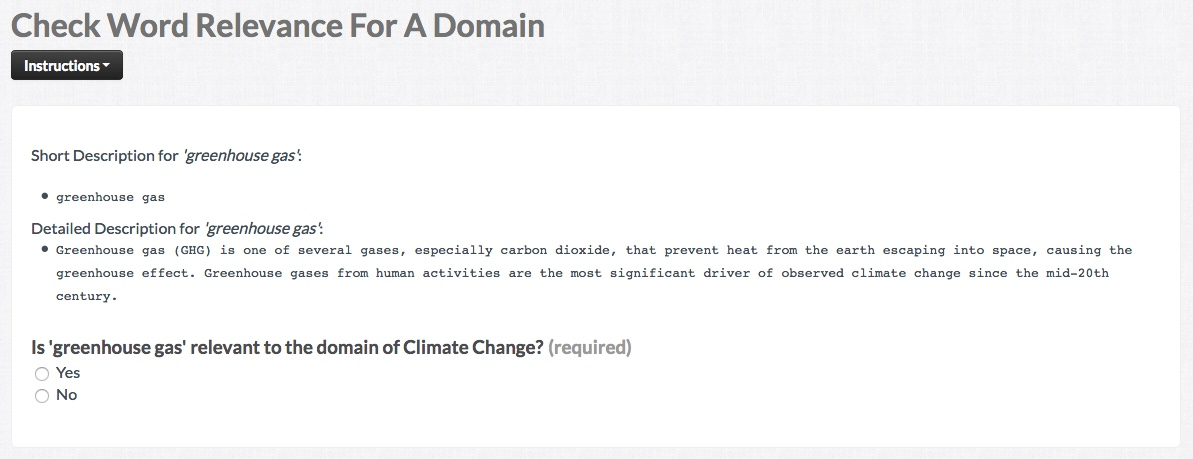
\includegraphics[width=\textwidth]{screenshots/questionaire_embedded_context_enrichment}
        \caption{Embedded Context}
        \label{fig:crowdsourcing_interface_ec}
    \end{subfigure}
	~\\~\\
    \begin{subfigure}[b]{\textwidth}
        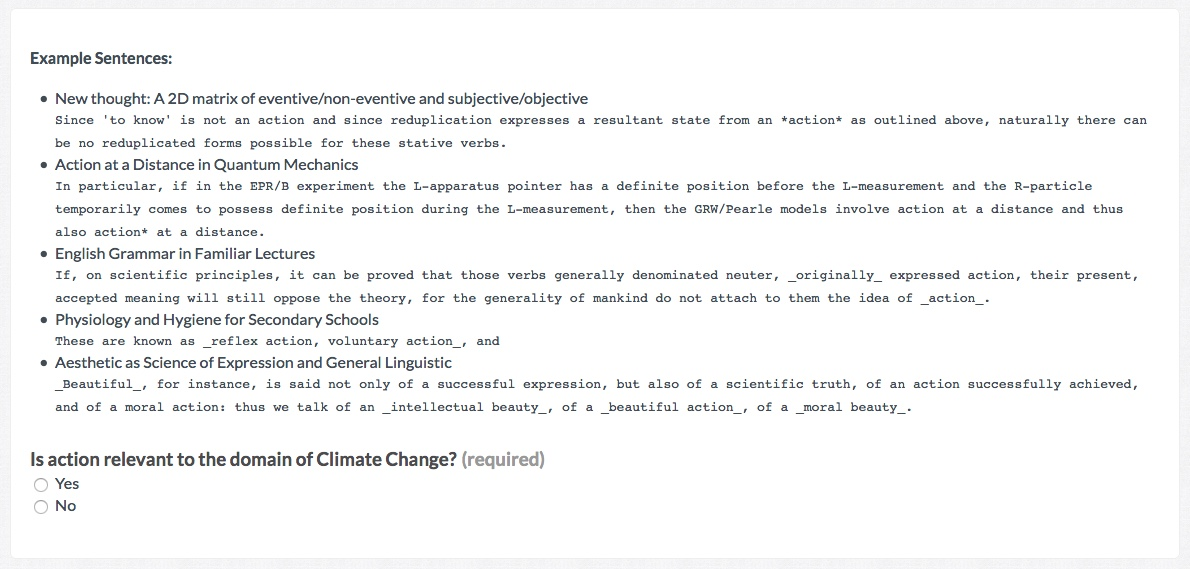
\includegraphics[width=\textwidth]{screenshots/questionaire_wordnik_context_enrichment}
        \caption{External Source}
        \label{fig:crowdsourcing_interface_es}
    \end{subfigure}
    \caption{Crowdsourcing task interfaces for performing ontology validation using different methods of context enrichment}\label{fig:all_crowdsourcing_interfaces}
\end{figure}

